\documentclass[10pt,a4paper,printanswers]{upmc} 

\usepackage[T1]{fontenc}
\usepackage[utf8]{inputenc}
\usepackage[english]{babel}
\usepackage{amsmath}
\usepackage{amssymb}
\usepackage[ruled,vlined,linesnumbered]{algorithm2e}
\usepackage{mathtools}
\usepackage[usenames,dvipsnames]{xcolor}
\usepackage{framed}
\usepackage[framemethod=tikz]{mdframed}
\usepackage{listings}         

\global\mdfdefinestyle{graybox}{%
  linecolor=black,linewidth=1pt,%
 % leftmargin=1cm,rightmargin=1cm,%
  backgroundcolor=lightgray
}

\mdfdefinestyle{evaluation}{
    frametitlebackgroundcolor=black!15,
    frametitlerule=true,
    roundcorner=10pt,
    middlelinewidth=1pt,
    innermargin=0.5cm,
    outermargin=0.5cm,
    innerleftmargin=0.5cm,
    innerrightmargin=0.5cm,
    innertopmargin=\topskip,
    innerbottommargin=\topskip,
    frametitle={Milestone}
}

\usepackage[textwidth=18cm,textheight=25cm]{geometry}

\newcommand{\myline}{\noindent\makebox[\linewidth]{\rule{\textwidth}{0.7pt}}}
\newcommand{\mytilde}{\raise.17ex\hbox{$\scriptstyle\mathtt{\sim}$}}

\newcounter{mainmemorder}
\newcommand{\save}{\setcounter{mainmemorder}{\value{enumi}}}
\newcommand{\load}{\setcounter{enumi}{\value{mainmemorder}}}
\newcommand{\mytext}[1]{\colorbox{lightgray}{\texttt{#1}}}
\newcommand{\subsecline}{\texorpdfstring{\hrulefill}{}}

\newcommand{\Num}{Part 1}
\newcommand{\UE}{\scriptsize M1 ISI/SAR/IPS\\ ROS \& experimental robotics}

\renewcommand*{\theenumi}{\#\thesubsection.\arabic{enumi}}

\title{ROS and experimental robotics.\\ \Num: an introduction to ROS.}


\lstset{language=matlab,
  basicstyle=\small\sffamily,
  keywordstyle=\color{dblue}\bfseries,  
  commentstyle=\color{dred}\textit,
  stringstyle=\color{dgreen}\ttfamily,
  extendedchars=true,
  frame=single, 
  numbers=left,
  backgroundcolor=\color{lgray}
}


\begin{document}

\maketitle

\section{ROS tutorial}
\label{sec:tutorial}
\vspace{-0.5cm}\myline\\

In addition to the first introduction courses (lasting 4h) you have, it is mandatory for you to
carefully follow the ROS tutorial indicated on Moodle as it will explain practically how ROS works,
its structure, its terminology, its basic commands and how to exploit \texttt{rospy} to actually
program your own ROS node.

This section constitutes thus a \textbf{mandatory homework}, and you have about \textbf{10 days} to
complete the entire tutorial (the precise dates will be given during the first presentation course
of the teaching unit). In the meantime, a discussion forum is made available on Moodle and all your
teachers will try respond as fast as possible to the questions you might have. Practically, we
recommend you to open the ROS tutorial on Firefox in the virtual machine, so that it will be easier
to copy/paste commands from the web page to your terminal. \textbf{Be careful: following the
  tutorial is not about copying and pasting commands, but rather about understanding the core concepts
  and understanding all the proposed linux/ROS commands.}

In the end of the tutorial period, your knowledge and understanding of ROS will be assessed through
multiple choice questions on Moodle.
\begin{mdframed}[style=graybox]
  The tutorial is available at
  \url{https://moodle-sciences.upmc.fr/moodle-2021/mod/page/view.php?id=130145}. Note that the
  creation of a ROS workspace mentioned in some tutorial (e.g.\ \texttt{Installing and}
  \texttt{configuring your ROS environment}) \textbf{is already done on the provided virtual
    machine}. So, your ROS workspace is located at \texttt{/home/turtle/catkin\_ws}.\\

  \noindent For the record, we will use the \textbf{\texttt{ROS 1 Noetic Ninjemys}} distribution in this
  teaching
  unit.\\

  \noindent At the end of this tutorial, you are supposed to precisely know:
  \begin{itemize}
    \itemsep=-1pt
    \item what are the root ROS concepts : nodes, messages, publishing and receiving messages,
          services, parameters;
    \item what is the architecture supporting these concepts: data structures, ROS master and all
          the servers running with it (parameter server, logging facilities, etc.),
          \mytext{roscore}, etc.;
    \item what is a ROS package, what it is made off,  what is the package build system used in ROS
          and how to use it;
    \item master the core shell commands that allow to investigate a ROS architecture
          (\mytext{rosnode}, \mytext{rosmsg}, \\\mytext{rostopic}, \mytext{rosservice},
          \mytext{roslaunch}, \mytext{rosrun}, etc.);
    \item and all the concepts highlighted during the first two courses (client/server applications,
          callback, etc.)
  \end{itemize}
\end{mdframed}
\newpage
\section{Practicals}
\vspace{-0.5cm}\myline\\

The two first practical sessions are devoted to the writing of your very first own ROS node. We will
gradually complexify the way it works, in order for you to deal with subscribing and publishing to
topics, exploiting services and the parameter server. At first, you will write a basic teleoperation
node which will capture the arrow keys of your keyboard so as to make the turtle from the
\texttt{tutlesim} package move on the screen. Then, we will complexify this example by changing the
color of the line following the turtle as a function of its position on the screen. Finally, we will
also change the color of the screen itself when the turtle is approaching each side of the screen
thanks to a parameter available in the parameter server.

One of the advantage of ROS is reusability. It means that the teleoperation node you will write to
move the turtle on your screen can also be used to move a real robot from your keyboard. Thanks to
the use of parameters and launch files, we will illustrate this by controlling a TurtleBot 3 burger
(see Figure~\ref{fig:turtlebot_family}) from the very same teleoperation node.

\begin{figure}[!h]
  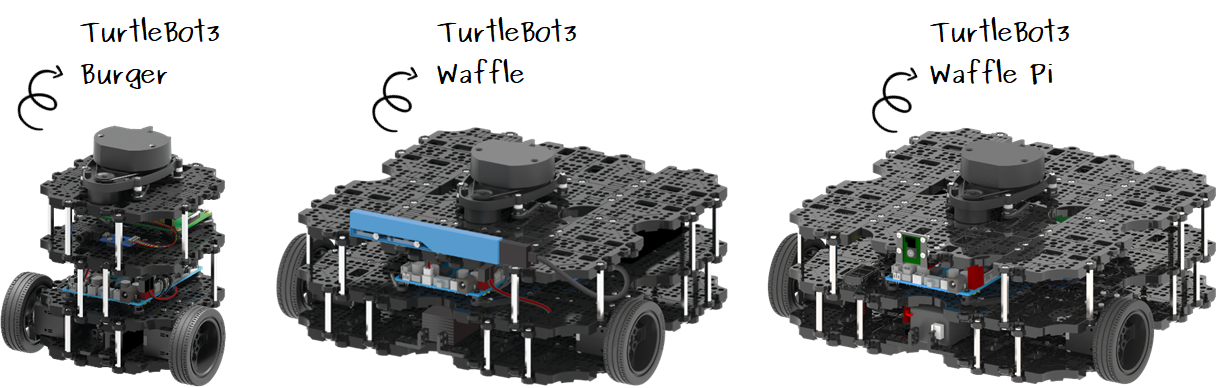
\includegraphics[width=\linewidth]{figures/turtlebot3_models.png}
  \caption{The entire TurtleBot 3 family. In this teaching unit, you will work with the small one,
    the TurtleBot3 Burger.}
  \label{fig:turtlebot_family}
\end{figure}

\begin{mdframed}[style=graybox]
  It is clear that all these tasks (working with topics, services, parameters and launch files) will
  require some times to be mastered. Nevertheless, most of these points will be reused in the Part 3
  of this teaching unit. So if you do not have the time to complete everything by the end of
  Part 1, you will have the opportunity to work on these concepts later.
\end{mdframed}

\subsection{Part A: a teleoperation node \subsecline}
\label{subsec:teleop_node}

In this first part, we will write a teleoperation node that aims at controlling the movement of the
turtle in the \texttt{turtlesim} package. All the forthcoming development will be based on
\texttt{Python}, and we will thus use the ROS client library \texttt{rospy} to interface with ROS.

\begin{mdframed}[style=graybox]
  \textbf{It is expected you already master Python syntax} (\textit{it should be the case thanks to
    the Python teaching unit from the first semester!}) as well as classical scientific libraries
  like \texttt{numpy} or \texttt{scipy}. If not, please refer to the documents provided during the
  first semester so that you will no transform this ROS class into a Python class.

  The \texttt{rospy} code API documentation is available at
  \url{http://docs.ros.org/api/rospy/html/}. A short tutoriel on \texttt{rospy} can be found at
  \url{http://wiki.ros.org/rospy/Overview}.
\end{mdframed}

\subsubsection{A look inside the \texttt{turtlesim\_node}} To begin with, we will run the
\texttt{turtlesim\_node} from the \texttt{turtlesim} package, and analyze its functioning before
sending data to make the turtle move. Of course, all the commands, code, etc. you will develop must
be written \emph{inside} the virtual machine (i.e.\ the remote PC) where ROS is already installed.
So please start it up before every practical sessions.

\begin{enumerate}
  \item From a Terminal, run the \texttt{turtlesim\_node} from the \texttt{turtlesim} package.
  \item List all the currently running nodes, and display information about the node
        \mytext{/turtlesim}. What kind of information is available?
  \item Now, list all of the currently active topics (i.e.\ topics where data are or can be sent or
        received). Indicate what topics are exposed by the \texttt{turtlesim\_node}, and who is
        subscribed or publishing to them.
  \item The turtle can be moved by sending appropriate messages to the topic
        \mytext{/turtle1/cmd\_vel}. Find out what kind of message (i.e. data type) is expected on
        this topic.
  \item Now that you know the expected message on \mytext{/turtle1/cmd\_vel}, display the message
        description to understand precisely what it is made of.
        \save
\end{enumerate}

\subsubsection{Creation of the \texttt{mybot\_teleop} package}

\begin{enumerate}
  \load
  \item Place yourself in the \texttt{src} folder of your ROS workspace, and create a ROS package
        called \texttt{mybot\_teleop} with dependencies to \texttt{std\_msgs} and \texttt{rospy}.
  \item Next go the newly created folder, and edit the file \texttt{package.xml} to enter your name
        as a developer. Finally, compile the new (empty) package. Do not forget, after compilation,
        to source the generated setup file \mytext{\mytilde/catkin\_ws/devel/setup.bash} (it has to
        be done only once, after the initial compilation, in all the currently opened terminal
        sessions).
  \item \label{item:executable}Download from Moodle the file \texttt{mybot\_teleop.py}, and place it
        inside a \texttt{scripts} folder inside the \texttt{mybot\_teleop} package. On the currently
        opened terminal, go to the \texttt{scripts} directory and make the Python script executable
        with the following commands: \lstinputlisting[
          %caption=Luftballons Perl Script, % Caption above the listing
          %label=lst:luftballons, % Label for referencing this listing
          language=bash, % Use Perl functions/syntax highlighting
          frame=single, % Frame around the code listing
          showstringspaces=false, % Don't put marks in string spaces
          numbers=left, % Line numbers on left
          numberstyle=\tiny, % Line numbers styling
          basicstyle=\footnotesize,
        ]{code/mybot_teleop_executable.shell}
        %
  \item Open the Python script \texttt{mybot\_teleop.py} in your favorite editor to visualize the
        code. You are now ready to write your first ROS node!
        \save
\end{enumerate}

%\newpage
\subsubsection{Creation of the \texttt{mybot\_teleop} node}
In this subsection, we will write a ROS node \mytext{/mybot\_teleop} which will talk to the
\mytext{/turtlesim} node through the \mytext{/turtle1/cmd\_vel} topic. Basically,
\mytext{/mybot\_teleop} is thus a very simple publisher node, similar to the one you already worked
on during the ROS tutorial in \S\ref{sec:tutorial}.

\begin{enumerate}
  \load
  \item Writing a simple publisher node requires the following steps. For each of them, you have to
        find the correct syntax in Python, that you will have to report in the
        \texttt{mybot\_teleop.py} script. Please keep in parallel open the ROS tutorial webpage
        dedicated to the "\textit{writing (of) a simple publisher and subscriber (Python)}".
        \begin{itemize}
          \item import the data type expected for the topic \mytext{/turtle1/cmd\_vel};
          \item define a publisher on the \mytext{/turtle1/cmd\_vel} topic with the imported data
                type on the step before;
          \item initialize a new node with name \texttt{mybot\_teleop};
          \item define a rate at which you would like the data to be published;
          \item as long as the ROS node is not shut down, and according to the key pressed on the
                keyboard, build an appropriate message and publish it on \mytext{/turtle1/cmd\_vel}
                to make the turtle move.
        \end{itemize}
\end{enumerate}


\begin{mdframed}[style=evaluation]
  Call your teacher at the end of this subsection to demonstrate the use of your
  teleoperation node. You will also be questioned on the basic shell commands exploited above to
  investigate the ROS architecture.
\end{mdframed}

\subsection{Part B: using services \subsecline}

In this subsection, we will write a second ROS node which will possibly run in parallel to the
previous teleoperation node. This time, this new node will subscribe to the \mytext{/turtle1/pose}
topic (which returns the position of the turtle on the screen) and modify the color of the line
behind it thanks to a call to the ROS service \mytext{/turtle1/set\_pen} made available by the
\mytext{turtlesim\_node}. Of course, you will have to run first the \mytext{turtlesim\_node} if it
is not already running.

\begin{enumerate}
  \item Like before, create a new package \mytext{mybot\_color} with the same dependencies as
        before. Edit the file \texttt{package.xml}, compile the new package, and source again the
        bash configuration in the \texttt{devel} folder of your \texttt{catkin} workspace.
  \item Create a \texttt{scripts} folder inside the new package, download the file
        \texttt{mybot\_color.py} from Moodle and place it inside the \texttt{scripts} folder. Do not
        forget to make the downloaded script executable! (see \ref{item:executable})
  \item List again of the available topics and study the expected message that should be received on
        \mytext{/turtle1/pose}.
  \item Writing a simple subscriber node requires the following steps. For each of them, you have to
        find the correct syntax in Python, that you will have to report in the
        \texttt{mybot\_color.py} script. Please keep in parallel open the ROS tutorial webpage
        dedicated to the "\textit{writing (of) a simple publisher and subscriber (Python)}".
        \begin{itemize}
          \item initialise a new ROS node with name \texttt{mybot\_color};
          \item import the data type expected for the topic \mytext{/turtle1/pose};
          \item define a subscriber on the \mytext{/turtle1/pose} topic with the imported data type
                on the step before together with a callback function which will be run each time a
                new data is present on the subscribed topic;
          \item and write the callback function for whatever you would like to do with the available
                data. For now, just print in the Terminal the \texttt{x} and \texttt{y} position of the
                turtle.
        \end{itemize}
        %
        \save
\end{enumerate}

Your are now able to get the \texttt{x} and \texttt{y} position of the turtle thanks to the
continuous reading of the \mytext{/turtle1/pose} topic. We want now to change the color of the line
following the turtle as a function of this position. As an example, we want to change the line to
red when approaching the edge of the screen. To do that, the \mytext{turtlesim\_node} exposes a
ROS service named \mytext{turtle1/set\_pen}.

\begin{enumerate}
  \load
  \item First, list all the services exposed by the \mytext{/turtlesim} node, and display
        information about the service\\ \mytext{turtle1/set\_pen}.
  \item Then display what data type is expected to be sent to the service \mytext{turtle1/set\_pen}
        and what kind of data will be returned.
  \item Writing a simple service client in a ROS node requires the following steps. For each of
        them, you have to find the correct syntax in Python, that you will have to add to the
        \texttt{mybot\_color.py} script. Please keep in parallel open the ROS tutorial webpage
        dedicated to the "\textit{writing (of) a Simple Service and Client (Python)}".
        \begin{itemize}
          \item first, import the data type expected to be sent to call the
                \mytext{turtle1/set\_pen} service.
          \item then use the \texttt{wait\_for\_service} method from \texttt{rospy} to wait for the
                service to be ready, and create a handle for calling the \mytext{/turtle1/set\_pen}
                service.
          \item and finally, use your handle wherever you need in the script, with the correct
                arguments, to call the service. For the record, the default pen values used in the
                turtlesim node are \texttt{r}=179, \texttt{g}=184, \texttt{b}=255, \texttt{width}=3,
                \texttt{off}=False. In this exercise, please try to make a minimal number of calls
                to the service (i.e. only when entering or leaving the corners of the screen).
        \end{itemize}
        \save
\end{enumerate}
At the end, you should have 4 terminals respectively occupied by \mytext{roscore}, the
\mytext{turtlesim\_node}, the \mytext{mybot\_teleop} node and the \mytext{mybot\_color} node. A
capture of one example of the expected outcome is shown in Figure~\ref{fig:turtlesim}.
\begin{figure}
  \centering 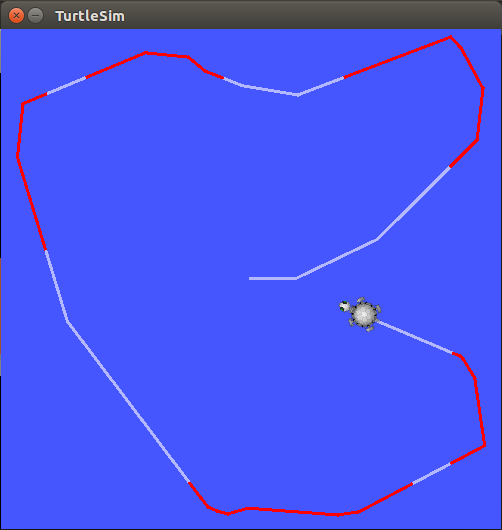
\includegraphics[width=6cm]{figures/turtlesim.png}
  \caption{A capture of the turtlesim view, where the line turns red when approaching the screen
    corners.}
  \label{fig:turtlesim}
\end{figure}

\begin{enumerate}
  \load
  \item Please validate your architecture with a \mytext{rqt\_graph} shown to your teacher, as well
        as a figure analog to Figure~\ref{fig:turtlesim}.
\end{enumerate}

\begin{mdframed}[style=evaluation]
  Call your teacher at the end of this subsection to demonstrate the use of your
  \mytext{mybot\_color} node. You will also be questioned on the basic shell commands exploited
  above to investigate the ROS architecture and your knowledge on ROS services.
\end{mdframed}


\newpage
\subsection{Part C: launchfile and parameters to teleoperate the Turtlebot 3 Burger \subsecline}

At the end of the previous part, you had to launch \textit{multiple nodes} by hand, each of them in
their own terminal. Launch files allow you to specify in one place all the nodes you would like to
run together. Additionnaly, this is a convenient place to write the values of some parameters of
your nodes, i.e.\ values in you code that can be changed at run time.

We will use launch files in the following to make the \mytext{mybot\_teleop} node generic, so that
you will be able to teleoperate a real robot with the very same ROS node than the one teleoperating
the turtlesim. Of course, the speed commands between the real robot and the turtlesim may differ:
this is where we will exploit parameters to change the value of the command accordingly.

\subsubsection{Using launch files to launch multiple nodes}
A launch file is a specific ROS file written using the XML format and specifying which nodes must
be run, with which arguments or parameters, eventually on which distant machine, etc. It is a very
powerful way to deal with very large scale ROS architectures, including a lot of ROS nodes with
their own parameters.

\begin{enumerate}
  \item First, download from Moodle the minimal launch file \mytext{turtlesim.launch} (see
        Listing~\ref{lst:launchfile} on page~\pageref{lst:launchfile}), and place it inside a new
        \texttt{launch} folder inside the \mytext{mybot\_teleop} package. Open it with your favorite
        code editor, and comment its content (see \url{http://wiki.ros.org/roslaunch/XML} for
        understanding the main options for the \texttt{<node>} XML tag).
  \item Run \emph{by hand} the \mytext{turtlesim\_node} in one terminal, and then use the previous
        launch file to run with \mytext{roslaunch} the \mytext{mybot\_teleop} node in a second
        terminal. You should able to teleoperate the turtlesim like in \S\ref{subsec:teleop_node}.
  \item Modify the launch file to automatically run the \mytext{turtlesim\_node} \emph{and} the
        \mytext{mybot\_teleop} node. Now, you can run both nodes with only one \mytext{roslaunch}
        command.
        \save
\end{enumerate}

%\newpage
\subsubsection{Using launchfiles to set parameters}
In the previous \mytext{mybot\_teleop} node, nothing can be tuned to adapt the node to the
teleoperation of anything different from the original turtlesim. For instance, if one wants to make
tunable the speed command sent to the robot when pressing a key on the keyboard, it is necessary to
modify the node code itself. Even if in this case this should not be a problem, we will benefit from
the possibility to define parameters in the launch file to make the \mytext{mybot\_teleop} node a
bit more generic.

A parameter server is launched together with the ROS master when running the \texttt{roscore}
command. It stores all the parameters of the currently running nodes, and a change of a parameter
value is made by sending a request to this parameter server.

\begin{enumerate}
  \load
  \item First, after running the \texttt{turtlesim\_node} and the \texttt{mybot\_teleop} node, list
        all available parameters.
  \item Next, thanks to the \texttt{<param>} tag, add two parameters with respective name
        \texttt{linear\_scale} and \texttt{angular\_scale} and values \texttt{1.0} to your
        \mytext{turtlesim.launch} file (see \url{http://wiki.ros.org/roslaunch/XML/param} for the
        exact syntax).
  \item After launching again the launch file, check if the two parameters are now correctly
        recorded in the parameters server.
        \save
\end{enumerate}

\newpage
The question is now: how can you get these two parameters values in your node code? The
client API \texttt{rospy} proposes one method \texttt{get\_param()} to get a parameter value from
its name.

\begin{enumerate}
  \load
  \item Adapt the script \texttt{mybot\_teleop.py} to get the parameters value from the parameters
        server, and check if everything is working as before (it should be the case!). You can then
        change the parameters values to higher or lower values and verify the effect on the turtle
        movement on the screen.
        \save
\end{enumerate}
\begin{mdframed}[style=evaluation]
  Call your teacher at the end of this subsection to demonstrate the use of your
  launch file. You will also be questioned on how you handled parameters in your ROS node.
\end{mdframed}


\subsubsection{Teleoperating the (simulated) Turtlebot3 burger}

We will now use the \mytext{mybot\_teleop} node to teleoperate a simulated Turtlebot 3 burger robot.
Working with a simulated realistic robot (or even a real robot!) is not different from listening and
subscribing to topics, using services, etc.\ like before, except that the node you are working with
is actually driving a simulated robot inside a physical simulator. The simulator we will be using in
all the following is \texttt{gazebo}. \texttt{gazebo} provides a robust physics engine, high-quality
graphics, and convenient programmatic and graphical interfaces to rapidly test algorithms, design
robots, perform regression testing, and train AI system using realistic scenarios. Interestingly,
\texttt{gazebo} works well with ROS and can be launched and controlled directly from it. You will
learn how to exploit \texttt{gazebo} together with a robot (physical) description and sensors in the
next chapter. In the meantime, we will use it here only as a convenient visualization tool allowing
you to simply see the robot movement in an empty world.

\begin{enumerate}
  \load
  \item To begin, launch the \mytext{turtlebot3\_empty\_world} launch file from the
        \mytext{turtlebot3\_gazebo} package. \\\texttt{gazebo} should now be running (the first
        launch might be long), and a simulated TurtleBot 3 Burger should appear at the center of the
        simulated (empty) world.
  \item List all currently running nodes and available topics. What is the name of the topic on
        which must be send the velocity command to make the robot move?
  \item From the previous step, one can see that the topic name used to send the velocity command is
        now different from the one used to command the turtlesim. Modify your code to account for this
        change by using an additional parameter set in a new launchfile \mytext{turtlebot.launch} you have
        to write (get inspiration from the previous one!). Then change the teleoperation node code to
        exploit this new parameter.
  \item Set the two parameters \texttt{linear\_scale} and \texttt{angular\_scale} to the appropriate
        values (to be determined!) in the \mytext{turtlebot.launch} launch file, and run the
        \mytext{mybot\_teleop} node. You should now be able to teleoperate the turtlebot!
  \item Finally, inspired by the \mytext{turtlebot3\_empty\_world.launch} file from the
        \mytext{turtlebot3\_gazebo} package, write your own \mytext{turtlebot3\_empty\_world.launch} file
        in charge of launching both \texttt{gazebo} \textit{and} your teleoperation node.
        \save
\end{enumerate}

\begin{mdframed}[style=evaluation]
  Call your teacher at the end of this subsection to demonstrate the teleoperation of the simulated
  Turtlebot 3 Burger.
\end{mdframed}

\subsubsection{Teleoperating the (real) Turtlebot3 burger}

\begin{enumerate}
  \load
  \item Read carefully the ``How-to operate the Turtlebot 3 burger'' document on Moodle, giving you
        all the steps required to setup and connect to the real robot. Ask your teacher a robot and
        try now to teleoperate it from the exact same \mytext{mybot\_teleop} node \ldots but you
        might again have to adapt the parameters to the robot (and this is actually all the point)!
\end{enumerate}

\newpage

\section*{Scripts to be completed}

\lstinputlisting[
  caption=mybot\_teleop.py script, % Caption above the listing
  %label=lst:luftballons, % Label for referencing this listing
  language=python, % Use Perl functions/syntax highlighting
  frame=single, % Frame around the code listing
  showstringspaces=false, % Don't put marks in string spaces
  numbers=left, % Line numbers on left
  numberstyle=\tiny, % Line numbers styling
  basicstyle=\footnotesize,
]{code/mybot_teleop.py}

\lstinputlisting[
  caption=mybot\_color.py script, % Caption above the listing
  %label=lst:luftballons, % Label for referencing this listing
  language=python, % Use Perl functions/syntax highlighting
  frame=single, % Frame around the code listing
  showstringspaces=false, % Don't put marks in string spaces
  numbers=left, % Line numbers on left
  numberstyle=\tiny, % Line numbers styling
  basicstyle=\footnotesize,
]{code/mybot_color.py}

\newpage
\lstinputlisting[
  caption=minimal turtlesim.launch script, % Caption above the listing
  label=lst:launchfile, % Label for referencing this listing
  language=xml, % Use Perl functions/syntax highlighting
  frame=single, % Frame around the code listing
  showstringspaces=false, % Don't put marks in string spaces
  numbers=left, % Line numbers on left
  numberstyle=\tiny, % Line numbers styling
  basicstyle=\footnotesize,
]{code/turtlesim.launch}

\end{document}
